\section{Expresiones regulares}

\subsection{Expresiones regulares (1)}
\begin{easylist}[itemize]
& Una expresión regular sobre un alfabeto usa los operadores binarios suma y producto y el operador unario estrella.

& El producto se denota sin escribir nada, y la estrella se expresa de forma similar a la exponenciación.

& Las expresiones básicas son, o bien símbolos del alfabeto, o bien $\Lambda$.

& Una expresión regular se interpreta como un lenguaje del siguiente modo:
    && Cada símbolo del alfabeto se interpreta como el lenguaje que sólo contiene ese símbolo.
    && El lenguaje de la palabra vacía, $\Lambda$, se interpreta como $\{\lambda\}$.
    && La suma se interpreta como unión.
    && El producto se interpreta como concatenación.
    && La estrella se interpreta como la operación estrella de lenguajes.

& Ejemplo: $a + bc^* (a + b)^* + \Lambda$ es una expresión regular que describe el lenguaje $\{a\} \cup [\{b\} \cdot \{c\}^* \cdot (\{a\} \cup \{b\})^*] \cup \{\lambda\}$.
    
& Así, las expresiones regulares son un método de representación de lenguajes. De hecho, de forma abusiva, identificaremos la expresión con el lenguaje representado.

& Es obvio que toda expresión regular representa un lenguaje regular, ya que los lenguajes regulares son cerrados por unión, concatenación y estrella, y existen autómatas triviales que reconocen a un solo símbolo o a la palabra vacía.

& Lo que no es tan obvio es que todo lenguaje regular se puede representar mediante una expresión regular. Es decir, para todo autómata existe una expresión regular que representa el lenguaje reconocido por el autómata. Para demostrar esto, necesitamos algunos contenidos teóricos.

& Suponemos la ecuación $X = AX + B$, donde $A$ y $B$ son lenguajes concretos y $X$ es una variable con rango en los lenguajes. Queremos saber las soluciones de la ecuación. Es decir, aquellos que, al sustituir $X$ por uno de ellos, hace la igualdad cierta.

& El \textit{lema de Arden} nos explica cómo tratar con esta igualdad en tres pasos.
&& La primera solución es $X = A^*B$.

    &&& Demostración: $A(A^*B) + B = A^+B + \Lambda B = (A^+ + \Lambda)B = A^* B$.

&& Cualquier otra solución $L$ contiene a $A^*B$. Esto es, $\forall L \colon (L = AL + B \implies A^*B \subseteq L)$.
    
    &&& Demostración: por cumplir la ecuación, $L$ contiene a $B$, $B \subseteq L$; por el mismo motivo $L$ contiene a $AL$ y, por tanto, a $AB$: $AB\subseteq AL \subseteq L$.
    
    &&& Similarmente, como $L$ contiene a $AL$ y a $AB$, entonces contiene a $A(AB)$, que es $A(A^2 B)$. Así, sucesivamente, vemos que $\forall n\colon(A^n B \subseteq L)$.
    &&& Esto concluye que $A^*B \subseteq L$.

&& Finalmente, vemos que, si $A$ no contiene la palabra vacía, entonces la única solución de la ecuación es $A^* B$. Esto es, $\lambda \notin A \implies \forall L \colon (L = AL + B \implies L = A^*B)$.
    
    &&& Lo demostramos por reducción al absurdo, suponiendo que $\lambda \notin A$, y que existe una solución a la ecuación diferente de $A^* B$: $L = AL + B \land L \neq A^* B$.
    
    &&& Como toda solución de la ecuación contiene a $A^* B$, para que $L$ y $A^*B$ sean distintos, tiene que haber una palabra $w$ que no esté en $A^* B$: $w \in L - A^* B$. Escogemos una palabra de longitud mínima ($|w|$ mínima) cumpliendo esta condición.
    
    &&& Por la ecuación, esto es $w \in (AL + B) - B$; pero, entonces, $w \in AL$.
    
    &&& Así pues, $w$ se puede construir por concatenación de una palabra de $w_1$ de $A$ con una palabra de $w_2$ de L.
    
    &&& Como $w \notin A^* B$ por hipótesis, entonces $w_w \notin A^* B$, y como $\lambda \notin A$, entonces $|w_2| < |w|$.
    
    &&& Así, hemos visto que $w_2 \in L - A^* B$, pero $|w_2| < |w|$. Esto contradice la elección mínima de $w$.
    
& Volvemos al objetivo principal: convertir un autómata en una expresión regular mediante un ejemplo.

& Queremos la expresión regular del lenguaje $L = \{w \in \{0,1\}^* \colon \mathrm{valor}_2 (w) \in \dot 3\}$; esto es, de las palabras binarias múltiples de 3.

& Su autómata es el siguiente.

\ \begin{tikzpicture}[->,>=stealth',shorten >=1pt,auto,node distance=2.8cm,semithick]

\node[initial, accepting, state] (A)  {$0$};
\node[state] (B) [right of=A] {$1$};
\node[state] (C) [right of=B] {$2$};


  \path (A) edge [loop above] node {$0$} (A)
        (C) edge [loop right] node {$1$} (C)
        (A) edge [bend left] node {$1$} (B)
        (B) edge [bend left] node {$1$} (A)
        (B) edge [bend left] node {$0$} (C)
        (C) edge [bend left] node {$0$} (B);
\end{tikzpicture}

& Llamemos a $L_0$ al lenguaje reconocido desde el estado $0$. De hecho, $L_0$ es el lenguaje de los múltiples de 3, ya que el estado 0 es el estado inicial. Similarmente, sean $L_1 = \mathcal L(A, 1)$ y $L_2 =\mathcal L (A, 2)$.

& Las palabras reconocidas desde el estado 0, o bien son la palabra vacía, ya que el estado 0 es aceptador, o bien empiezan por 0 y vienen seguidas de una palabra aceptada empezando desde el estado 0, o bien empiezan por 1 y vienen seguidas de una palabra aceptada empezando desde el estado 1. Esto es: $L_0 = \Lambda + 0 L_0 + 1 L_1$.

& Similarmente, las palabras reconocidas desde el estado 1 no pueden ser la palabra vacía ya que el estado aceptador. Y, o bien empiezan por 0 y vienen seguidas a continuación de una palabra aceptada empezando por el estado 2, o bien empiezan por 1 y vienen seguidas de una palabra aceptada empezando por el estado 0. $L_1 = 0 L_2 + 1 L_0$.

& Análogamente, $L_2 = 0L_1 + 1 L_2$.

& Esto las tres ecuaciones anteriores nos garantizan que $L_0$, $L_1$ y $L_2$ forman una solución de este sistema de ecuaciones:

\Deactivate
$$\begin{array}{lcl}
X_0 &=& \Lambda + 0 X_0 + 1 X_1\\
X_1 &=& 0X_2 + 1 X_0\\
X_2 &=& 0X_1 + 1X_2\end{array}$$
\Activate

& Vamos a aprovechar el lema de Arden para aislar las variables, ver que la solución es única y obtener una expresión regular del lenguaje reconocido por el autómata.

&& Aplicando el lema de Arden, podemos aislar $X_2$ de la última ecuación así: $X_2 = 1^* 0X_1$. Nótese que el $1$ juega el papel del lenguaje $A$ que no contiene la palabra vacía, y $0X_1$ juega el papel de $B$.

&& Sustituyendo $X_2$ en la segunda ecuación, tenemos que $X_1 = 01^* 0X_1 + 1X_0$. Si aplicamos el lema de Arden, tenemos que $X_1 = (01^* 0)^* 1 X_0$.

&& Sustituyendo $X_1$ por la expresión anterior en la primera ecuación, tenemos que $X_0 = \Lambda + 0 X_0 + 1(01^*0)^* 1 X_0 = \Lambda + (0 + 1(01^*0)^* 1) X_0$, por distributividad de suma y producto.

&& Aplicando, de nuevo, el lema de Arden, $$X_0 = (0 + 1(01^* 0)^* 1)^* \Lambda = (0 + 1(01^* 0)^* 1)^*.$$

&& Esta es, pues, la expresión regular que representa los múltiples de 3.
\end{easylist}

\subsection{Expresiones regulares (2)}
\begin{easylist}[itemize]
& Una expresión regular se puede convertir en una gramática que genere el mismo lenguaje de un modo muy sencillo, ya que los lenguajes incontextuales están cerrados por unión, concatenación y estrella, que son, precisamente, las operaciones que nos permiten construir las expresiones regulares.

& La transformación a partir del ejemplo anterior, es decir, $(0 + 1(01^*0)^* 1)^*$ es

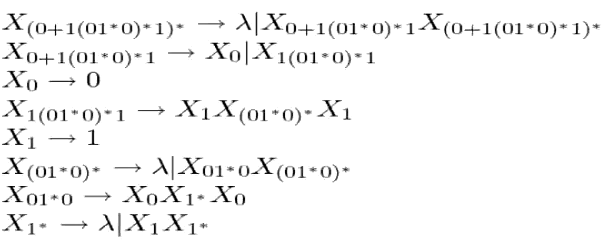
\includegraphics{t3-2.png}

& Para todo lenguaje regular, existe una gramática que lo genera. Es decir, la clase de los lenguajes regulares está incluida dentro de la clase de los lenguajes incontextuales.

& Hay una manera más sencilla de obtener una gramática a partir de un autómata que es más directa.

& Este es el autómata de los múltiples de 3.

\ \begin{tikzpicture}[->,>=stealth',shorten >=1pt,auto,node distance=2.8cm,semithick]

\node[initial, accepting, state] (A)  {$0$};
\node[state] (B) [right of=A] {$1$};
\node[state] (C) [right of=B] {$2$};


  \path (A) edge [loop above] node {$0$} (A)
        (C) edge [loop right] node {$1$} (C)
        (A) edge [bend left] node {$1$} (B)
        (B) edge [bend left] node {$1$} (A)
        (B) edge [bend left] node {$0$} (C)
        (C) edge [bend left] node {$0$} (B);
\end{tikzpicture}


& Y esta es la gramática que obtenemos a partir de él:

\Deactivate
$$\begin{array}{lcl}
X_0 &\to& \lambda | 0X_0 | 1X_1\\
X_1 &\to& 0X_2 | 1X_0\\
X_2 &\to& 0X_1 | 1X_2\end{array}$$
\Activate


& Tenemos una variable de la gramática para cada estado del autómata ($X_0$, $X_1$ y $X_2$). El objetivo de $X_0$ es generar todas las palabras que nos llevan a estado aceptador empezando la ejecución desde el estado 0. Y lo mismo para $X_1$ y $X_2$.

& Las palabras que nos llevan a estado aceptador desde el estado $0$ o bien son la palabra vacía (porque el estado es aceptador), o bien empiezan por $0$ y vienen seguidas de una palabra que nos lleva desde el estado $0$ al estado aceptador, o bien empiezan por $1$ y vienen seguidas de una palabra que nos lleva desde el estado $1$ al estado aceptador. Lo mismo sucede para $X_1$ y $X_2$. En estos dos últimos casos, no aceptamos la palabra vacía porque no son estados aceptadores.

& Por la construcción de la gramática, resulta obvio que genera el lenguaje reconocido por el autómata. Un argumento inductivo nos permitiría demostrarlo. De hecho, esta gramática simula el autómata.

& Considérese la ejecución aceptadora $$q_0 10101 = q_1 0101 = q_2 101 = q_2 01 = q_1 1 = q_0.$$

& Mediante la derivación $$X_0 \to_G 1X_1 \to_G 10X_2 \to_G 101X_2 \to_G 1010X_1 \to_G 10101X_0 \to_G 10101,$$ la gramática genera la misma palabra a base de ir recordando el estado en el que se encuentra el autómata con la palabra leída hasta el momento. Las $\lambda$-producciones, que tan solo aparecen en las variables de estados aceptadores, nos permiten terminar la derivación.

& Las gramáticas tales que cada parte derecha de regla tiene como mucho una variable, y donde esta aparece cuanto más a la derecha posible se denominan gramáticas lineales por la derecha, o gramáticas regulares por la derecha. Este tipo de gramáticas siempre generan lenguajes regulares.

& Existe una transformación similar de autómatas en gramáticas lineales por la izquierda, también llamadas gramáticas regulares por la izquierda. Estas se definen de manera análoga.
\end{easylist}